%!TEX root = ../thesis.tex
% NIR-information

\chapter{Information content of \nir{} Spectra}
\label{cha:nir_content}

The work presented in this chapter focuses on calculating and analysing the information content of stellar spectra, specifically the radial velocity precision in the \nir{}.
This work is not directly related to detecting exoplanet atmospheres themselves but investigates the theoretical and observed {RV} precision of {M-dwarf} spectra in the \nir{}.
Aiding future detections of the detection of future
This can help in detecting the presence of ``habitable Earth-like'' planets around {M-dwarfs} which could become prime targets for future exoplanet atmosphere studies.

The field of exoplanet detection in the \nir{} is expanding with several new high-resolution \nir{} spectrographs becoming available in the near future (see \cref{subsec:new_generation}).
One science objective common to all four instruments is the detection of small mass planets around {M-dwarf} stars utilizing the radial velocity technique.
The fundamental radial velocity precision of {M-dwarf} spectra attainable at different wavelength regions calculated in~\citet{figueira_radial_2016} was used to influence some design choices of {SPIRou}, {NIRPS}.
For instance {NIRPS} opted not to cover the \emph{K}-band, favouring a higher spectral resolution and simplicity, but preserved the possibility for adding a K-band spectrograph in a separate cyrostat in the future.

The purpose of the work presented in this chapter is to extend the work of~\citet{figueira_radial_2016}, computing the theoretical RV precision of stellar spectra over a wider range of situations.
An investigation into the effect of \logg{} and \feh{} on precision is performed and a comparison of RV precision of the recently observed \nir{} {M-dwarf} spectra from {CARMENES} library and their synthetic counterparts will be performed.
This is to test how the {RV} precision of synthetic models compares to reality.
The aim is to compare the fundamental precision of observed \nir{} spectra to the synthetic models.


\section{Overview}
\todo{remove duplication}
The pursuit of detecting exoplanets, especially ``habitable'' and ``Earth-like'' planets, requires state-of-the-art instrumentation with high precision.
One of the key detection methods, the Radial Velocity ({RV}) method, measures the wobble induced on the Star by the planet as they orbit their common barycentre \reference{rv method}.  {\red{} add Some stuff about mass and period from Pedros paper}  \todo{put in introduction??}

\todo{derivation of rv?}

The number of \nir{} spectrographs focusing on cooler {M-dwarfs} stars is increasing, which have a relatively better chance of detecting Earth-like planets in the habitable zone.
This work continues the assessment of {RV} precision levels possible in the \nir{} domain, an extension of~\citep{figueira_radial_2016}.

\missingfigure{An example from Figueira et al.
2016}


\citet{artigau_optical_2018} recently compared archival spectra of Barnard's Star, an {M-dwarf}, and found that state-of-the-art atmosphere models over-predict the \emph{Y}- and \emph{J}-band {RV} content by more than a factor of \(\sim2\), while under-predicting the \emph{H} and \emph{K}-band content by half.
{\red{} in this work we find similar?}

This has previously helped to aid the direction of instrument design by identifying the wavelength regions with the best {RV} precision~\citep{figueira_radial_2016} but can also help in the planning of observations, by understanding how the precision changes with spectral type and observed {\snr{}}.


\textbf{THIS is from spie 2018 conference.}
{red{} \citep{quirrenbach_carmenes_2018} With this strategy it has been possible to achieve 1--2 m/s precision in the visible and 5--10 m/s precision in the {near-IR}; further improvements are expected from ongoing work on temperature control, calibration procedures and data reduction. Comparing the RV precision achieved in different wavelength bands, we find a ``sweet spot'' between 0.7 and 0.8\um, where deep \ce{TiO} bands provide rich RV information in mid-M dwarfs. This is in contrast to our pre-survey models, which predicted comparatively better performance in the near-IR around 1\um, and explains in part why our near-IR RVs do not reach the same precision level as those taken with the visible spectrograph.}




\subsection{Fundamental photon noise limitation}
\label{subsec:fundamental_precision}
A technique to calculate the theoretical radial velocity precision of a spectrum using the full spectral information in an optimal way was presented by~\citet{connes_absolute_1985}.
Here we provide the radial velocity precision derivation following~\citet{connes_absolute_1985, bouchy_fundamental_2001, figueira_radial_2016}.
A majority of this derivation follows~\citet{bouchy_fundamental_2001} with extra explanations and notes added.

\begin{figure}
    \centering
    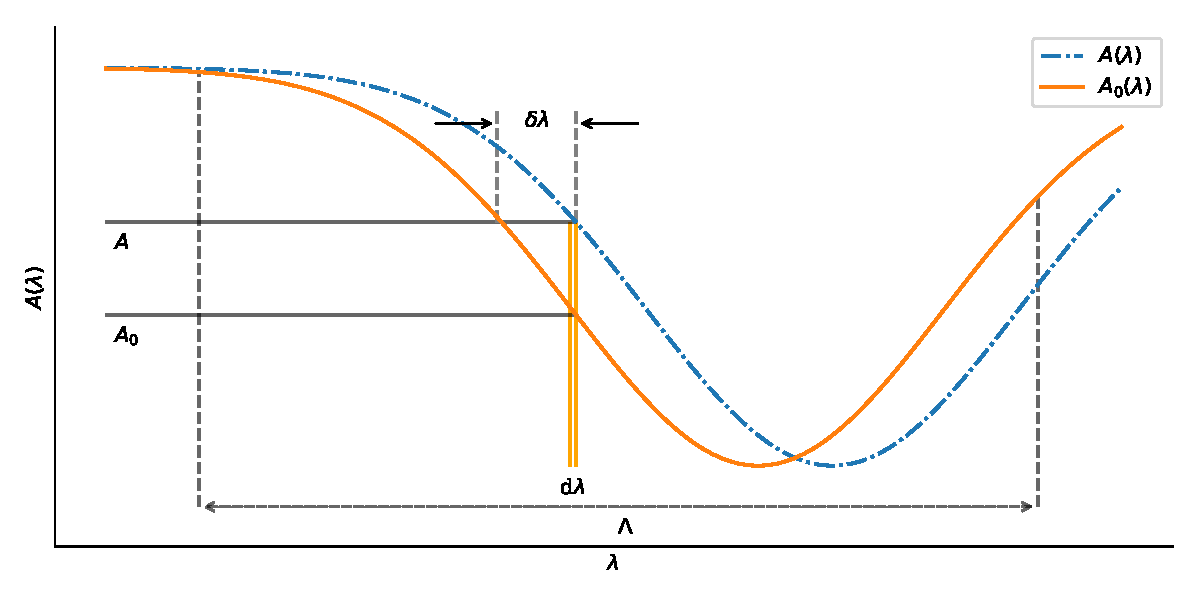
\includegraphics[width=0.7\linewidth]{figures/information-content/precision_plot.pdf}
    \caption[Demonstration of a shifted arbitrary spectral line.]{Arbitrary spectral line with a shift \(\delta \lambda\), inspired by~\citet{connes_absolute_1985}.  \(\Lambda\) is the wavelength range considered.}
    \label{fig:precisionderivation}
\end{figure}
\todo{add \(\delta A\) to plots}

For demonstration purposes  \cref{fig:precisionderivation} show a portion of an arbitrary spectrum \(A(\lambda)\), for demonstration purposes over a wavelength range \(\Lambda\).
Here \(A_0(\lambda)\) is the reference spectrum while \(A(\lambda)\) is observed some later time with an apparent wavelength shift observed.
It shows most of a single Gaussian line as spectral lines contain the most information but the requirement of spectral lines is not a requirement.

The Doppler shift of a spectrum is given by:
\begin{equation}
\frac{\delta V}{c} = \frac{\delta \lambda}{\lambda},
\label{eqn:dopplershift}
\end{equation}
where \(c\) is the speed of light in a vacuum, and \(\delta \lambda\) is the shift in wavelength \(\lambda\) due to the velocity \(\delta V\).

\todo{intensity change from connes is vertically in the slice d lambda}

Using basic calculus \(\delta y = \pd{y}{x} \delta x \nonumber\), and for a Doppler shift that is small compared to the line-width\footnote{Although~\citet{connes_absolute_1985} show that the approximation in \cref{eqn:intensitychange} is adequate under all circumstances}, the observable intensity change in a wavelength slice \(d \lambda\) (or at a given pixel) can be expressed by:
\begin{equation}
\delta A(i) = A(i) - A_0(i) \simeq \pd{A_0(i)}{\lambda(i)} \delta \lambda.
\label{eqn:intensitychange}
\end{equation}

Rearranging \cref{eqn:intensitychange} for \(\delta \lambda\) and combining it with \cref{eqn:dopplershift}, the Doppler shift of then becomes:
\begin{equation}
    \frac{\delta V(i)}{c} = \frac{A(i) - A_0(i) }{\lambda(i) (\partial A_0(i)/\partial \lambda(i))} \label{eqn:delta_v_i}
\end{equation}

This equation shows that the radial velocity measured at pixel, i, through a change in the intensity in the recorded spectrum, \(A(i)-A_0(i)\), and inversely proportional to the slope of the spectrum, \({\partial A_0(i)}/{\partial \lambda(i)}\).
\Cref{eqn:delta_v_i} provides a separate measurement of the radial velocity shift for every pixel, $i$, in the spectrum.
The sensitivity of the velocity measurement can be improved, and the noise decreased by using the information from the whole spectral range, \(\Lambda\).
This is achieved by taking the weighted average\footnote{Weighted average on x is \(\bar{x} = \frac{\sum{ x(i)W(i)}}{\sum {W(i)}}\)} over all pixels in the spectral range using an optimal pixel weight \(W(i)\).

\begin{equation}
\bar{\frac{\delta V}{c}} = \frac{\sum{\frac{\delta V(i)}{c}W(i)}}{\sum {W(i)}}.
\end{equation}

Statistically, the optimal weights are proportional to the inverse square of the individual dispersion (variance),
\begin{equation}
W(i) = \frac{1}{{\left(\frac{\delta V_{\rms}(i)}{c}\right)}^{2}}, \label{eqn:weights}
\end{equation}
where \(X_{\rms}\) is the dispersion on the quantity \(X\).

The individual dispersion of the velocity measurement \(\delta V_{\rms}(i)\) is the dispersion that would result from several measurements of the reference spectrum all with the same Doppler shift (e.g.\ zero). \Cref{eqn:delta_v_i} thus becomes:
\begin{equation}
    \frac{\delta V_{\rms}(i)}{c} = \frac{{[A(i) - A_0(i)]}_{\rms} }{\lambda(i) (\partial A_0(i)/\partial \lambda(i))}. \label{eqn:delta_v_i_rms}
\end{equation}
The noise of the spectrum A is the quadratic sum of the photon noise \(\sqrt{A}\) and the detector noise \(\sigma_D\).
The spectrum \(A_0\) is considered noise free.

\begin{equation}
{[{A(i)-A_0(i)}]}_{\rms} = {[{A(i)} - 0]}_{\rms} = \sqrt{{\sqrt{A(i)}}^{2} + {{\sigma}^{2}}_{D}} \label{eqn:noise}
\end{equation}

Considering that the Doppler shift is small and that \(A\) and \(A_0\) have the same intensity level, then \(A = A_0\) can be set.
Using \cref{eqn:delta_v_i,eqn:weights,eqn:noise} the optimum weights then become solely dependent on the reference spectrum.

\begin{equation}
W(i) = \frac{{\lambda}^{2}(i) {({\partial A_0(i)}/{\partial \lambda(i)})}^{2}}{A(i) + {\sigma}^{2}_{D}} \label{eqn:optimal_weight}
\end{equation}

This weighting function can be modified to mask out and eliminate unwanted lines in the spectrum.
For instance in the removal of telluric absorption lines in observed spectra.
This is achieved to setting the particular pixel weights to zero.

With the optimal weights set, the weighed average velocity change measured from the full spectral range \(\Lambda\), is given by:

\begin{eqnarray}
    \frac{\overline{\delta V}}{c} &= \frac{
        \sum{
            \frac{
                A(i) - A_0(i)}{
                \lambda(i) \left({\partial A_0(i)}/{\partial \lambda(i)}\right)} W(i)}}{
             \sum{{W(i)}}} \\
    &= \frac{
        \sum {
            (\frac
                {A(i) - A_0(i)}
                {\lambda(i) (\partial A_0(i)/\partial \lambda(i))}) \frac
                    {{\lambda}^{2}(i) {({\partial A_0(i)}/{\partial \lambda(i)})}^{2}}
                    {A_{0}(i) + {\sigma}^{2}_{D}}
                 }
         }
    {\frac
        {{\lambda}^{2}(i) {({\partial A_0(i)}/{\partial \lambda(i)})}^{2}}{A_{0}(i) + {{\sigma}^{2}}_{D}}
        } \\
    &= \\
    &= \frac{\sum{(A(i) - A_0(i)){\left(\frac{W(i)}{A_0 +{\sigma}_{D}^{2}}\right)}^{1/2}}}{\sum{W(i)}}
    \label{eqn:delta_v_eqarray}
\end{eqnarray}\unfinished{Finish this equation (9 of bouchy 2001)}
\unfinished{Try the symbolic package from PC}

The important quantity for {RV} measurements is not just the velocity values themselves but also the dispersion on the measured velocity, the RV precision, \(\delta V_{\rms}\), from the spectrum.
This allows one to assess the planetary detectability limitations attainable in the spectra.
From rearranging \cref{eqn:weights} the dispersion is given by:
\begin{equation}
    \overline{\frac{\delta V_{\rms}}{c}} = \frac{1}{\sqrt{\sum{\,W(i)}}} = \frac{1}{Q \sqrt{\sum{\,A_0(i)}}}. \label{eqn:dv_rms}
\end{equation}
With this the velocity precision is inversely proportional to the sum of the optimal pixel weights.

A spectral quality factor, Q, is defined as for the pure photon noise case in~\cite{connes_absolute_1985, connes_demonstration_1996}, as:
\begin{equation}
Q = \frac{\sqrt{\sum{\,W(i)}}}{\sqrt{\sum{\,A_0(i)}}}.
\end{equation}

The radial velocity precision or uncertainty can be rearranged in terms of the spectral quality;
\begin{equation}
    \delta V_{\rms} = \frac{c}{Q \sqrt{\sum {\,A_0(i)}}} = \frac{c}{Q \sqrt{{N}_{{e}^{-}}}} \approx \frac{c}{Q \cdot \snr{}},  \label{eqn:snr_relation}
\end{equation}
where \(\sum A_0(i) = {N}_{{e}^{-}}\) is considered to be the total number of photo-electrons \({N}_{{e}^{-}}\) counted in the spectral range considered.\todo{explain snr}{where the \({\snr{}}=\sqrt{N_{{e}^{-}}}\) for large N}
where the \({\snr{}}=\sqrt{N_{{e}^{-}}}\)for large N. \unfinished{It is convenient to use this version when comparing observed spectra with different \snr{}.?}


This quality factor, Q, is flux independent and is purely a function of the spectral profile within the spectral range considered.
It is a measure of the line richness i.e., quantity and depth.
For example a spectrum with many sharp lines will have a high Q.
This quality factor is valid for the pure photon noise case only in which \(\sigma_{D} =0\) and \({[A(i)]}_{\rms} = A_0\).
The instrumental resolution of the spectrograph also effects the spectral quality as it induces line broadening.

The number of photo-electrons counted \(N_{{e}^{-}}\) depends on the stellar magnitude, detector efficiency and integration time.
It can be estimated using
\begin{equation}
     N_{{e}^{-}} = P_{avg} * S_{tel} * \texp * \alpha* \Lambda,
\end{equation}
where \(P_{avg}\) is the average monochromatic stellar brightness
across the wavelength range \(\Lambda\) in \si{\photons\per\second\per\centi\metre\squared\per\centi\metre},
\(S_{tel}\) is the telescope collecting area in \si{\centi\metre\squared},
\(\texp\) is the integration time in \si{\second},

and \(\alpha\) the overall efficiency (including atmosphere, telescope, spectrograph and detector).

This can be used to determine the {RV} precision for a given instrument, and be useful in exposure time calculators for planning observations for RV surveys and exoplanet detection.

In the case of several \(\delta V\) measurements computed for \(k\) spectral slices (or spectral orders) then the error on the average \(\overline{\delta V}\) is given by the error on a weighted average:
\begin{equation}
\overline{\delta {V}_{\rms}} = \frac{1}{\sqrt{\sum_k{{(\frac{1}{\delta V_{\rms}(k)})}^{2}}}}  \label{eqn:weighted_average_error}
\end{equation}

This work follows~\cite{figueira_radial_2016} by exclusively considering a high signal-to-noise regime in which \({A(i) + \sigma_{D}^{2}} \sim {A(i)}\) can be approximated.


\footnote{pure detector noise the fluctuation are independent of the spectrum \(A\) and the quality factor for pure detector noise is \(Q_D = \frac{\sum{{\lambda}^{2} {(\partial A_0(i)/\partial \lambda(i))}^{2}}}{\sum{\, A_0(i)}}\) as derived by~\cite{connes_absolute_1985}. }


This technique has been tested and demonstrated on observations by~\citet{connes_demonstration_1996} and been used to determine predict the accuracy or performance limits of spectrograph instrumentation~\citep[e.g.][]{connes_absolute_1985,bouchy_fundamental_2001} and can influence the design (and/or use) of spectrographs
 (e.g.\ SPIROU~\citep{artigau_spirou_2014,figueira_radial_2016})
\unfinished{Does spectrograph pipelines such as HARPS use these equations to measure estimate/precision?}


Considering that \(\sum{A_0(i)} = N_{{e}^{-}}\)is the total number of photoelectrons counted over the whole spectral range then the uncertainty in the velocity change is finally given by:
\begin{equation}
\delta V_{\rms} = \frac{c}{Q \sqrt{N_{{e}^{-}}}} \approx \frac{c}{Q (\snr{})}, \label{eqn:rv_SNR}
\end{equation}
where the \(\snr{}=\sqrt{N_{{e}^{-}}}\)for large N. \unfinished{It is convenient to use this version when comparing observed spectra with different \snr{}.?}


In the unrealistic case where all the pixel weights are identical $W(i)=w$, then we can also see that the precision with decreases as $1/\sqrt{N}$ due to an increase in the number of pixels, or a increase in spectral range.
 \begin{equation}
 \delta V_{\rms} = \frac{c}{\sum{W(i)}} \approx \frac{c}{\sqrt{N w}}=  \frac{c}{\sqrt{N}\sqrt{w}}, \label{eqn:sqrtN}
 \end{equation}

A separate general formula for RV precision is given by~\citet{hatzes_spectrograph_1992} in terms of general spectral parameters.
\begin{equation}
\sigma = \frac{1}{\sqrt{F} \sqrt{\Lambda} {R}^{1.5}}
\end{equation}

Here the $\sqrt{F}$ represents the \snr{} of the spectrum in the possion-noise dominated regime.
The $\Lambda$ comes from assuming a homogenous distribution of line, with the same line properties, per unit length.



\subsection{Prepare {PHOENIX} aces models}:
\# see~\citet{figueira_radial_2016}

Convert SED to counts.


Scale to 100 \snr{} per resolution element in \emph{J}-band.

Convolutions

\subsection{Rotational convolution}
\label{subsec:rotational_convolution}
Stellar rotation has the affect of broadening spectral lines as the different portions of the stellar surface have a variation of radial velocity between \(\pm v \sin i\).
Rotation is applied to a non-rotating spectrum by convolution with a rotation kernel.
The stellar rotational kernel used is given by~\citet{gray_observation_2005};

\todo{top view diagram of rotation?}

\begin{align}
G(\Delta\lambda) &= \frac{2(1-\epsilon){[1-{(\Delta\lambda /{\Delta\lambda}_{L})}^{2}]}^{1/2} +   \frac{1}{2}\pi\epsilon[1-{(\Delta\lambda /{\Delta\lambda}_{L})}^{2}]}{\pi (1-\epsilon/3) \vsini}\\
      &= c_{1}{[1- {(\Delta\lambda /\Delta\lambda_{L})}^{2}]}^{1/2} + c_{2}[1-{(\Delta\lambda /\Delta\lambda_{L})}^{2}] \label{eqn:rotational_profile}
\end{align}
where
\begin{equation}
c_1 = \frac{2(1-\epsilon)} {\pi (1-\epsilon/3)\vsini},  \hspace{4em} c_2 = \frac{\frac{1}{2}\pi\epsilon} {\pi (1-\epsilon/3)\vsini},
\end{equation}
are constants which depend on the equatorial rotational velocity \Vsini{}.

Here $\Delta\lambda$ is the wavelength position from the non-rotating line centre, $\Delta\lambda_{L}$ is the maximum line shift of the line centre at the edge of the stellar disk at which point the Doppler shift is  \Vsini{}; $\Delta\lambda_{L} = \lambda \frac{\vsini}{c}$.

This kernel arises from integrating the rotational velocity profile across the surface of the stellar disk and as such the rotation kernel is bounded in the range  $[-\Delta\lambda_L, \Delta\lambda_{L}]$ from the line centre.
This kernel also accounts for limb-darkening on the stellar disk with the linear limb darkening coefficient used in this work fixed at $\epsilon=0.6$ as done in~\citet{figueira_radial_2016}.

Since the synthetic models do not have a consistent wavelength grid, the discretization of applying the convolution kernel onto the changing wavelength grid causes the result of each pixel to be multiplied by a slightly different kernel area.
Therefore, the result is divided by a convolution of a spectrum of ones with the same wavelength resolution to normalize the convolution.

As the Doppler shift \Vsini{} is transformed into wavelength by multiplication of $\lambda  / c$ there is a wavelength dependence on the rotation kernel shape.
That is, the rotation kernel at each pixel is unique and requires separate calculation.
For small wavelength ranges this can be held fixed to improve performance.
This simplifications is not performed in this work as large wavelength ranges are considered.


\subsection{Instrumental Convolution}
Following the rotational convolution the spectra are convolved with Gaussian instrumental profile ({\textrm{IP}}) with the {\fwhm}  constrained by the spectral resolution R, $\fwhm= \lambda/R$.

The Gaussian convolution kernel is of the form
\begin{equation}
IP(\Delta\lambda) = \frac{1}{\sigma \sqrt{2\pi}} \exp^{-\frac{{\Delta\lambda}^{2}}{2 {\sigma}^{2}}}    \label{eqn:IP_profile}
\end{equation}
with $\sigma = \frac{\fwhm}{2\sqrt{2 \ln(2)}}$, and $\Delta \lambda$ again the difference from the line centre (normally this would be written as $(x-\mu)$ where $\mu$ is the Gaussian centre).

This assumes that the instrument profile of a particular instrument is in-fact Gaussian.
This assumption of a Gaussian instrumental profile is a good starting point for high-resolution spectrographs, and shown to be valid for CRIRES~\citep{seifahrt_synthesising_2010}.
If the instrument profile of a particular instrument is well characterized, then it could replace the Gaussian profile used here.

For instance~\citet{artigau_optical_2018}  state that the instrumental profile of a (circular) fibre-fed spectrograph such as {HARPS} is mathematically equivalent to a cosine between $-\frac{\pi}{2}$ and $\frac{\pi}{2}$ with a width equivalent to the Gaussian {\fwhm}.

The integration of a circular fibre is given by
\begin{equation}
\textrm{IP}_{\textrm{fibre}(\Delta\lambda)} = \cos(B\cdot\Delta\lambda) ,  \hspace{2em} [-\frac{\pi}{2 B}, \frac{\pi}{2 B}]
\end{equation}
where {$B = \frac{\fwhm_{0}}{\fwhm}$ } is scaled to give the same area,
following the description from~\citet{artigau_optical_2018}.  They also mention that the result using this $\textrm{IP}_{\textrm{fibre}}$ are all consistent with just using a Gaussian kernel.

\subsection{Numerical Convolution}
\label{subsec:numerical_convolution}
In this work the stellar models undergo broadening by convolution with rotation and instrumental profile kernels (\cref{eqn:rotational_profile,eqn:IP_profile}).
The convolutions are performed by analysing a single pixel at a time, and selecting the neighbouring pixels that fall within the convolution window\footnote{Region in which the convolution kernel will affect this particular pixel} for that pixel.
The value of the convolution kernel is calculated at the position of each pixel selected, multiplied by the flux of each pixel and then summed to provide the new value at the selected single pixel{$^{\textbf{*}}$}.
 The shape of the convolution kernels and the size of convolution window are wavelength dependant (${\fwhm}=\lambda / R$ and $\Delta\lambda_{L}=\lambda \frac{\vsini}{c}$) and must be calculated separately for each pixel, making the convolution computationally expensive.

However, the computation of the convolution of individual pixels is an ``embarrassingly parallel''\footnote{\href{https://en.wikipedia.org/wiki/Embarrassingly\_parallel}{https://en.wikipedia.org/wiki/Embarrassingly\_parallel}} problem.
What this means is that convolution result for pixel $i+1$ does not depend on the convolution result obtained for pixel $i$.
Therefore, parallel processing was implemented to improve the performance of the convolution, roughly dividing the convolution time by the number of processors used.

The python package \emph{PyAstronomy} also contains functions that perform rotational and instrumental broadening.
Those functions however require that the spectrum have uniformly spaced $x$-coordinate spacing which is not a requirement for the implementation of \emph{eniric} used here. \emph{PyAstronomy}, while implemented a ``slow'' full version of the rotational convolution, with a wavelength dependent kernel, they also provide ``fast'' convolution kernels that are fixed, taking the central wavelength value.
These are significantly faster but are only valid for very short wavelength regions, in which the kernels do not significantly change.
They are not suitable for use in this work due to the large wavelength span of spectroscopic bands and the wavelength dependant spacing of the spectra.
A comparison of the performance between \emph{PyAstronomy} convolution and the convolutions implemented in \emph{eniric} and used here are given in a \emph{Jupyter} notebook in the repository of ``eniric'', basically they fall in between the ``fast'' and ``slow'' implementation of \emph{PyAstronomy}.

One factor the needs consideration when convolving with an non-uniformly spaced spectrum is effect of the sampling on the convolution.
For instance the number of point inside the convolution, as well as their location will effect the area of the convolution kernel.
To normalize the convolution result it is divided by the convolution of a unitary spectrum of ones, with the same spacing.
\citet{figueira_radial_2016} performed this unitary convolution separately and applied the normalization afterwards.
In the improved implementation the convolution normalization is performed directly after the convolution kernel multiplication at \(\textbf{*}\).

For example for the rotational convolution result of the value for pixel $i$ becomes
\[{A}^{\prime}(\lambda_{i}) =  \frac{\sum A(\Delta\lambda_{i}) \cdot G(\Delta\lambda_{i})}{\sum G(\Delta\lambda_{i})},\]
where $\Delta\lambda_{i}$ are the values between in the range $\lambda_{i} (1-\frac{\vsini}{c}) \le\lambda_{i} \le \lambda_{i} (1+ \frac{\vsini}{c})$,
instead of only
\[{A}^{\prime}(\lambda_{i}) =  \sum A(\Delta\lambda_{i}) \cdot G(\Delta\lambda_{i}).\]


By default edge effects are avoided by providing an input spectra sufficiently wider than the desired output spectrum to prevent edge effects on the portion of the spectrum desired.
Since two convolutions are preformed one after the other the original input spectrum is selected wider than needed so that no edge effects will be present after both addition of rotation and instrumental broadening by \Vsini{} and R.

%-----------------------------------
%    SUBSECTION 2
%-----------------------------------
\section{}
Preparation of {CARMENES} spectra.


\missingfigure{Example of {CARMENES} spectra before and after correction}

\subsection{Bands}
The bands analysed avoid the strong water absorption in the \nir{} that can be seen the {CARMENES} spectra in Figure~\reference{Add figure here}\todo{Add figure here}. These are the Z, Y, J, H, K- bands found in \cref{tab:infrared_bands}.


\subsection{Comparing models to {CARMENES}.}
Already somewhat done in Reiners. (use all spectra).
They measured the precision obtained in the spectra.

Band by band like~\citet{figueira_radial_2016}?
Certain\% steps like Bouchy or Artigau


Can do Barnard's star in {CARMENES}. \todo{finish this} compared to models in Artigau.

\DTLsetseparator{,}
\DTLloadrawdb{targets}{data/carmenes_selection.csv}%

\begin{table*}[h]
    \centering
    \caption[Selection of targets from the {CARMENES} library.]{Selection of targets from the {CARMENES} library spanning the {M-dwarf} spectral range.}
    \begin{tabular}{l l l r c c c c}%
        \toprule
        Karmn & Name & SpT &  \({\snr{}}_{\textrm{NIR}}\)  & Temp (K)  & \logg{} & \feh{} & v\(\sin{i}\) (\kmps{})\\
        \midrule
        \DTLforeach*{targets}{\id=Karmn,\name=Name,\sptype=SpT,\SNR=NIR-SNR,\TEFF=Teff, \LOGG=logg,\metal=FeH, \rot=ROT-Vsini}{
            \DTLiffirstrow{}{\\}\id{} & \name{}  & \sptype{} & \SNR{} & \TEFF{} & \LOGG{} & \metal{} & \rot{}
        }
        \\
        \bottomrule
    \end{tabular}
    \label{tab:targets}
\end{table*}

%!TEX root = ../thesis.tex

\begin{table}[h]
    \caption{csv2tex table}
    \begin{tabular}{lllrrrrr}
        \toprule
        Karmn &            Name &   SpT &  NIR-SNR &    Teff &  logg &   FeH &  ROT-Vsini \\
        \midrule
        J20533+621 &      BD+61 2068 &  M0.5 &      257 &  3772.0 &     - & -0.01 &       2.66 \\
        J04290+219 &       BD+21 652 &  M0.5 &      212 &  4037.0 &  3.99 & -0.21 &       1.11 \\
        J07274+052 &   Luyten's Star &  M3.5 &      254 &  3467.0 &     - & -0.11 &          - \\
        J17578+046 &  Barnard's Star &  M3.5 &      236 &  3247.0 &     - & -0.32 &          - \\
        J11055+435 &          WX UMa &  M5.5 &      140 &  3304.0 &     - &     - &          - \\
        J10564+070 &          CN Leo &  M6.0 &      133 &  2960.0 &     - &     - &          - \\
        J18356+329 &  LSR J1835+3259 &  M8.5 &       50 &  2578.0 &     - & -0.40 &      37.60 \\
        J04198+425 &  LSR J0419+4233 &  M8.5 &       42 &       - &     - &  0.22 &          - \\
    \bottomrule
    \end{tabular}\label{tab:carmenes_selection}
\end{table}

%\begin{table}
\label{}
\caption{csv2tex table transposed}
\begin{tabular}{lllllllll}
\toprule
{} &           0 &           1 &              2 &               3 &           4 &           5 &               6 &               7 \\
\midrule
Karmn     &  J20533+621 &  J04290+219 &     J07274+052 &      J17578+046 &  J11055+435 &  J10564+070 &      J18356+329 &      J04198+425 \\
Name      &  BD+61 2068 &   BD+21 652 &  Luyten's Star &  Barnard's Star &      WX UMa &      CN Leo &  LSR J1835+3259 &  LSR J0419+4233 \\
SpT       &        M0.5 &        M0.5 &           M3.5 &            M3.5 &        M5.5 &        M6.0 &            M8.5 &            M8.5 \\
NIR-SNR   &         257 &         212 &            254 &             236 &         140 &         133 &              50 &              42 \\
Teff      &        3772 &        4037 &           3467 &            3247 &        3304 &        2960 &            2578 &               - \\
logg      &           - &        3.99 &              - &               - &           - &           - &               - &               - \\
FeH       &       -0.01 &       -0.21 &          -0.11 &           -0.32 &           - &           - &            -0.4 &            0.22 \\
ROT-Vsini &        2.66 &        1.11 &              - &               - &           - &           - &            37.6 &               - \\
\bottomrule
\end{tabular}
\end{table}


\section{Metallicity \logg{} effects}
We explore the effect of metallicity and \logg{} on the spectral quality of spectra in the {PHOENIX-ACES} library by extending the quality factor and precisions computation to \feh{} between -1--1 and \logg{} of 4.0--5.5.
In \cref{fig:deviations} the variation of quality factor with broadening of R=100\,000 and $\vsini=1.0$\kmps{} across the {M-dwarf} spectral types and the \nir{} bands is shown.
We observed multiple different effects present.


The \emph{Z}-band has a large separation in spectral quality due to spectral type, this is because the continuum the \emph{Z}-band is severely eroded in the spectra of late M's as they cool.
Each spectral type also behaves very differently to a change in \feh{} and \logg{}.
For {M0} and {M3} there is an increase with \feh{} below solar metallicity, above solar metallicity the slopes of the lines dramatically increase, especially for {M3}.
For {M6} and {M9} there is a step slope with \feh{} below solar metallicity, which flattens off at solar metallicity, and even decreases for the {M9} spectra above solar metallicity.
As \logg{} increases in the \emph{Z}-band there is a decrease in quality.
There is a consistently large separation between early and late M's that.
The quality for {M6} is very shallow, while for {M9} the quality is nearly flat for \logg{}=4.0 and 4.5 but then decreases sharply at higher \logg{}.

\emph{Y}-band -\\

\emph{J}-band - \\

For the H and \emph{K}-band there is fairly consistent linear trend for all spectral types, with the quality factor increasing with an increase in \feh{} and decreasing with an increase in \logg{}.
There is also only a relatively small variation in quality factor due to the spectral type.



\begin{figure}
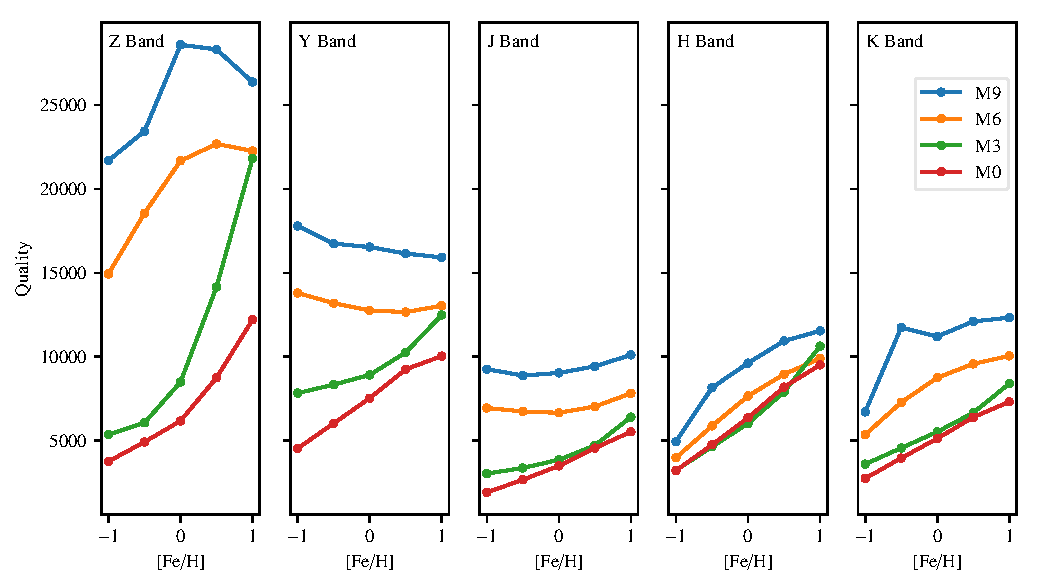
\includegraphics[width=0.99\linewidth]{figures/information-content/metalicity_effect.pdf}\\
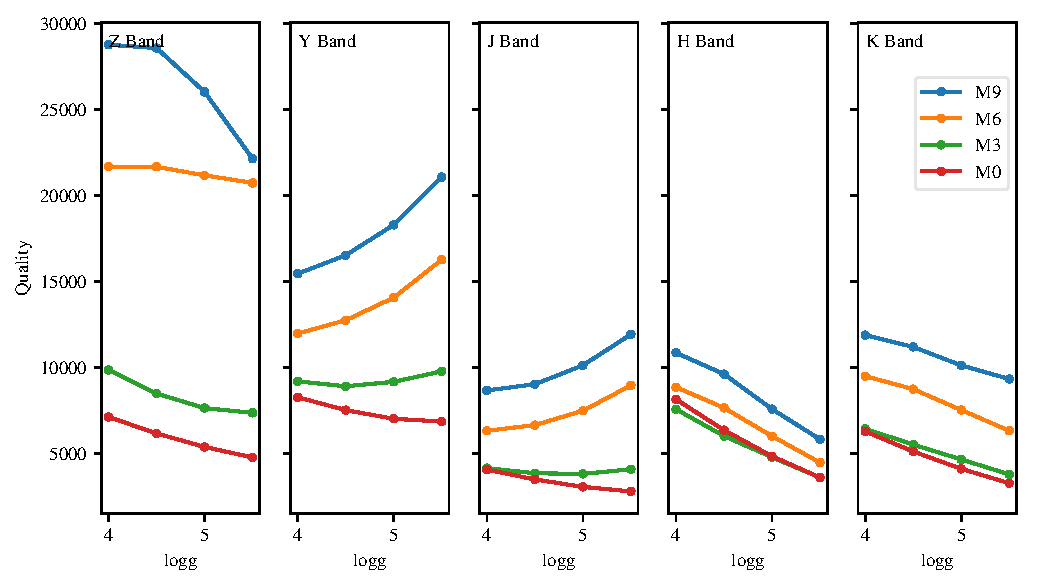
\includegraphics[width=0.99\linewidth]{figures/information-content/logg_effect.pdf}
\caption[Quality factor verse \feh{} and \logg{} for different spectral types and wavelength bands.]{Quality factor changes across spectral type and bands for variations in \feh{} and \logg{}.
Broadening values are R=100\,000 and \Vsini{} = 1.0\kmps{}.
Top: Quality factor variation of \feh{} between -1.0 to 1.0 at a fixed \logg{}=4.5.
Bottom: Quality factor variation of \logg{} between 4 and 5.5 with fixed \feh{}=0.0.
Note a higher quality factor corresponds to an increased {RV} precision.}
\label{fig:deviations}
\end{figure}


\clearpage

\section{Updating {RV} precision software}
To undertake the calculation of RV precisions
A large section of this work involved optimizing the original code used in~\citet{figueira_radial_2016}.
Care needs to be taken to optimize the code.
The original code used in~\citet{figueira_radial_2016} was slow, taking around 2 hours per simulation, this led to multiple weeks of processing time to compute the precision's for the original paper.

In this section we document the changes made to the code in the course of attempting to improving it.
Features that change the derived {RV} precision are specifically documented in detail, with relative precision changes provided.

This work resulted in a submission of a publication\footnote{Available at \href{http://joss.theoj.org/papers/384bfc031df47ecef2d88328f63e5479}{http://joss.theoj.org/papers/384bfc031df47ecef2d88328f63e5479}} to \emph{The Journal of Open Source Software}\footnote{\href{http://joss.theoj.org/}{joss.theoj.org/}} (JOSS) {Neal and Figueria 2018 (in prep.)} with the source code openly available on \href{Github}{https://github.com/jason-neal/eniric}.


\subsection{Automated testing}
To insure that any changes made to the code did not change the underling results.
This involved writing automatic tests for the software.
This practice is crucial in computer science ins commercial software development but seldom done in research but is becoming more popular. \reference{works of software testing in research.}
Some work focused on testing ideology from computer science.
Although not perfect implementation I began by adding automated tests to the code to check individual parts of it.
Before making changes I created automated tests that would confirm the functionality of pieces of the code.
I could then make changes to the code, to improve the performance without worrying that the results were different.
Namely that the same precision were calculated in the end.

Functional test and unit tests.


\subsection{Performance}
\label{subsec:code_performance}
There was a major performance bottleneck in the convolution stage, which increased the performance around 250\,X itself.
The algorithm looped though the pixels in the spectrum, selecting out the necessary section around a given pixel with a comprehension list (for loop if inside range).
Turning the result into a \emph{numpy} array, performing the sum for that pixel and appending it to a list.
The performance issue was a python implementation detail to do with applying a comprehension list to a \emph{numpy} array, then slicing the \emph{numpy} array with the ends of the list, then converting it back into a \emph{numpy} array, all of which is preformed on a very large spectrum array.
Creating a \emph{numpy} boolean mask instead of the comprehension list, and applying the boolean mask to the array is much faster.
Remaining entirely in the compiled \emph{numpy} code and not converting between lists and \emph{numpy} arrays (with involve type checking overhead).
This slow operation was done for every pixel/wavelength in the spectrum twice, once for each convolution.

caching convolution result to prevent recomputing the same values. \emph{Joblib}.  Also embarrassingly parallel so added multiprocessing support.

The convolution is still the slowest part.
There are other methods that work on uniform spectra, which have not been tried to see how they affect the performance or {RV} precision results.
\textbf{Insert code samples.}


\subsection{Model extension}
The solution is to iterate over each pixel but create a mask array and use \emph{numpy} indexing to select the required pixel span. (this remains in \emph{numpy})
These operations all remain in \emph{numpy} so do not waste time converting between lists and \emph{numpy} arrays, in which Python need to constantly check and convert the type of each item.

This shows a lesson in the usefulness of test driven development, or testing of code in science.


An normalization step was originally done after the convolution, to normalize out the effect of the convolution on a spectrum of 1s, due to the changing wavelength grids sampling.
This was brought inside the main convolution by dividing the pixel by the convolution of a spectrum of ones at the same time. (again in \emph{numpy} so it is quick)

Parallelization as embarrassingly parallel, the result of each pixel is independent of result of neighbours.

This is not a criticism of the work done by the original author (my supervisor).
It is easier to modify a working system then to create one from scratch.

Computer code is not the important part in scientific exploration., although becoming more important in open source and reproducibility efforts.
Often forgotten in

\# Handle any {PHOENIX} aces models.


\section{Numerical Gradient}
\label{sec:numerical_gradient}
One of the key insights from \cref{eqn:optimal_weight,eqn:dv_rms} is that the radial velocity error is inversely proportional gradient of the spectra, In numerically computing the {RV} precision, the result is dependent on the numerical method used to compute the gradient.
In original code used in~\citet{figueira_radial_2016} the gradient or slope is approximated using the forward finite difference method.
The \emph{numpy} package provides a function to calculate the gradient using a more advanced methods that compute a more precise gradient.
In this section we explore the affect of improving the precision of the numerical gradient on the final {RV} precision.

The simplest way to calculate the derivative using finite difference methods~\citep{quarteroni_numerical_2000}.
These arising from the Newton's definition of the derivative for a continuous function \(f(x)\) which should be familiar from introductory calculus:
\[f'(x) = \lim_{h \to 0} \frac{f(x+h)-f(x)}{h}~.\]

There are three common varieties of the finite difference,
\begin{equation}
 {FFD} = \frac{f(x+h)-f(x)}{h}, {CFD}=\frac{f(x+\frac{1}{2}h)-f(x-\frac{1}{2}h)}{h}, {BFD}=\frac{f(x)-f(x-h)}{h}\,,
\end{equation}
called the forwards ({FFD}), central ({CFD}), and backwards ({BFD}) finite differences respectively.
The order of uncertainty on the {FFD}/{BFD} is \(\mathcal{O}(h)\) while for the {CFD} it is \(\mathcal{O}({h}^{2})\)~\citep{quarteroni_numerical_2000}.
As the wavelength spacing between samples/pixels (h) is small the {CFD} will a more precise value for the gradient at each pixel.

In our case \(h\) is the difference in wavelength between the two pixels considered.
In the {FFD} case the gradient at pixel \(i\) becomes:
\begin{equation}
\frac{\partial A_0(i)}{\partial\lambda(i)} = \frac{A_0(i+1) - A_0(i)}{\lambda(i+1)-\lambda(i)}, \hspace{2em} 1 \leq i \leq n-1.
\label{eqn:ffd_precision}
\end{equation}
At each pixel the numerical derivative is evaluated to the average slope between itself and the following pixel and is an approximation to the derivative.
This only extends to \(i= n-1\), where \(n\) is the number of points in the spectrum, and the last pixel is dropped from the {RV} calculation.\footnote{This is important in the case of Condition~\#2.}


The \emph{gradient}\footnote{Documentation available at \href{https://docs.scipy.org/doc/numpy/reference/generated/numpy.gradient.html\#id1 }{https://docs.scipy.org/doc/numpy/reference/generated/numpy.gradient.html\#id1}}  method provided in \emph{numpy} contains a more advanced numerical methods to calculate the derivative.
It uses a \textit{compact difference} method~\citep{quarteroni_numerical_2000} which expand the finite differences using a Taylor expansion and then selecting coefficients to minimize the \textit{consistency error}.
From the \emph{numpy} documentation the consistency error here is \[\eta_i = \partial{f(x_i)}/\partial{x} -  [\alpha f(x_i) + \beta f(x_i +h_d) + \gamma f(x_i - h_s)],\] where \(h_s\) and \(h_d\) are the spacing to the left and right of \(i\) respectively.
With Taylor expansion this turns into solving a linear system of equations:
\[\begin{cases}
         \alpha + \beta + \gamma = 0\\
         -\beta {h_d} + \gamma {h_s} = 1\\
         \beta {h_{d}}^{2} + \gamma {h_{s}}^{2} = 0
    \end{cases}
\]
which result in the approximation of the gradient of the central values to be

\[\frac{\partial{f(x_i)}}{\partial{x}} = \frac{{h_{s}}^{2}f\left(x_{i} + {h_{d}}\right) + \left({h_{d}}^{2} - {h_{s}}^{2}\right)f\left(x_{i}\right) - {h_{d}}^{2}f\left(x_{i}-{h_{s}}\right)} {{h_{s}}{h_{d}}\left({h_{d}} + {h_{s}}\right)} + \mathcal{O}\left(\frac{h_{d}{h_{s}}^{2} + {h_{s}}{h_{d}}^{2}}{{h_{d}} + {h_{s}}}\right) \label{full_compact_difference}.\]

If the spectrum is evenly spaced ${h_{s}}={h_{d}}$  reduces to the standard second order {CFD} approximation:

\[\frac{\partial{f(x_i)}}{\partial{x}} = \frac{f\left(x_{i+1}\right) - f\left(x_{i-1}\right)}{2h} + \mathcal{O}\left({h}^{2}\right)\]


Applying this to our situation, similar to \cref{eqn:ffd_precision}, we get:
\[\frac{\partial A_0(i)}{\partial\lambda(i)} = \frac{{\lambda(i-1)}^{2} A_0(i+1) + ({\lambda(i+1)}^{2}-{\lambda(i-1)}^{2}) A_0(i) - {\lambda(i+1)}^{2} A_0(i-1)} {\lambda(i-1)\lambda(i+1)(\lambda(i+1) + \lambda(i-1))}, \hspace{1em} 2 \leq i \leq n-1\]

with an uncertainty of \(\mathcal{O}\left(\frac{\lambda(i+1){\lambda(i-1)}^{2} + \lambda(i-1){\lambda(i+1)}^{2}}{\lambda(i+1) + \lambda(i-1)}\right)\).


{\red{} Wavelength spacing \(\delta\lambda\) between pixels is a function of \(\lambda\), Resolution and sampling choices.
Can I do something with this??}

The \emph{gradient} function from \emph{numpy} implements central differences for the interior points, accurate to second order, and first order accurate one-sided (forward or backward) differences at the boundaries, computed using the same compact difference procedure.

\begin{figure}
    \centering
    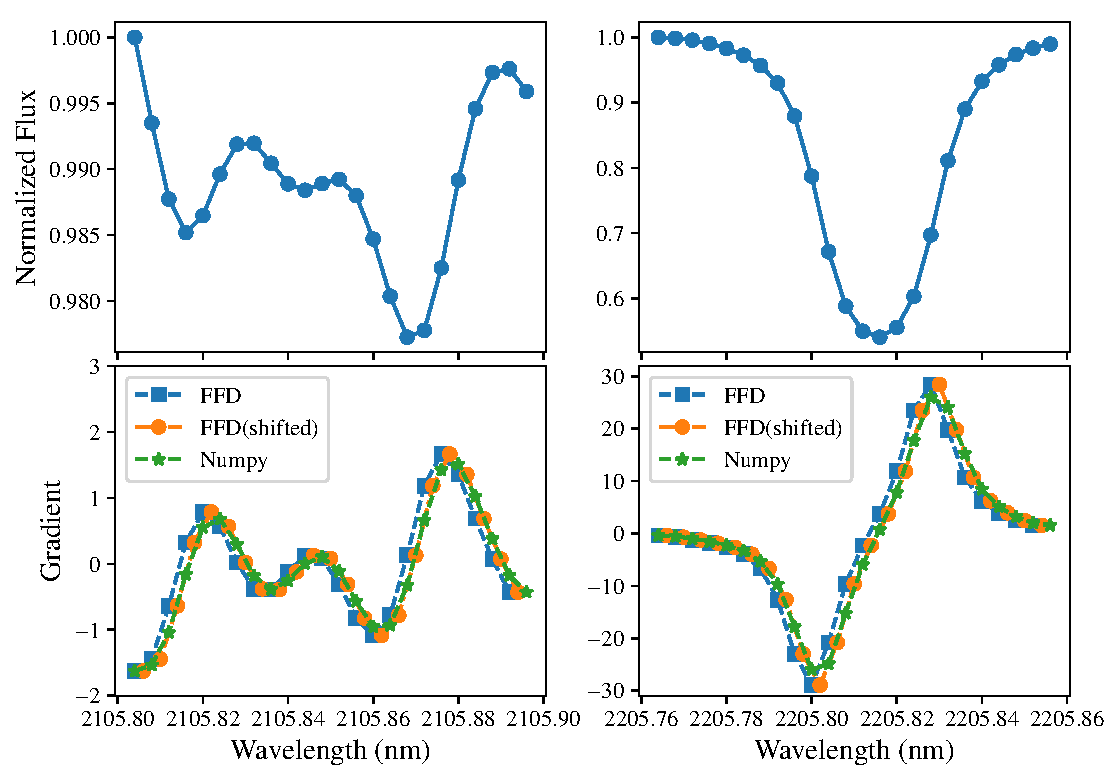
\includegraphics[width=0.8\linewidth]{figures/information-content/spectral_gradients}\\
    \caption[Comparing of numerical gradient alogithms.]{Visualization of the numerical gradient of some spectral lines.
        Top: The two spectral regions of a stellar spectrum the left hand slide contains short lines near the normalized continuum while on the right a single deep absorption line is shown.
        Bottom: The numerical gradients for the spectra shown in the top panels; the original {FFD} method is displayed with \emph{blue squares} while \emph{numpy} gradient is shown with \emph{green stars}.
        The \emph{orange circles} are the {FFD} version shifted to the mid-points between pixels for illustrative purposes.}
    \label{fig:gradients}
\end{figure}


%!TEX root = ../thesis.tex

\begin{table}
    \caption{The affect of the numerical gradient function on RV precision. The band label \(\rm VIS\) indicates the visible band while  \(\rm CARM_{VIS}\)  and \(\rm CARM_{NIR}\)  indicate the two wavelength bands of the CARMENES spectrograph. \(\Delta\lambda\) is a wavelength shift applied to analyse the pixel weights at the middle of their FFD gradients for comparison only.}
    \begin{tabular}{ccccccc}
        \toprule
%% Band & $\lambda$ range\_min & wl\_max &  dy/dx   & gradient & Q(dy/dx) & Q(grad) & Q(frac) & RV(dy/dx) & RV\_adj &    RV(grad)    &    RV(frac\_grad)    & RV(frac\_adj)          \\
  &   $\lambda$ range & \multicolumn{3}{c}{RV\(_{rms}\) (\mps{})} & \(\Delta\) RV ratio& \(\Delta\) RV ratio\\
 Gradient method&  &  A &   B & C & (B-A)/A & (C-A)/A \\
 Band  &  \si{\micro\meter} & FFD & FFD+\(\Delta\lambda\) &  CFD &  \% & \% \\
    \midrule
VIS & 0.38 -- 0.78 & 16.1 & 16.2 & 16.9  & 0.6 & 4.9\\
\(\rm CARM_{VIS}\) & 0.52 --  0.96 & 20.9 & 21.0 & 22.0 & 0.3& 5.2 \\
Z & 0.83 -- 0.93 & 76.9 & 77.0 & 78.8  & 0.1 & 2.5\\
Y & 1.00 -- 1.10 & 78.3 & 78.5 & 83.8 & 0.2 & 7.0 \\
J & 1.17 -- 1.33 & 149.3 & 149.4 & 156.4 & 0.1 & 4.7 \\
H & 1.50 -- 1.75 & 119.4 & 119.5 & 122.3 & 0.1 & 2.5 \\
K & 2.07 -- 2.35 & 153.4 & 153.7 & 157.7  & 0.2 & 2.8\\
\(\rm CARM_{NIR}\) & 0.96 -- 1.71 & 46.1 & 46.2 & 48.0 & 0.1& 4.2 \\
NIR & 0.83 -- 2.35 & 36.9 & 36.9 & 38.2 & 0.1 & 3.6  \\
    \bottomrule
    \end{tabular}\label{tab:numerical_gradients}
\end{table}


In \cref{fig:gradients} we visualize the gradients of two small spectral regions computed with the original {FFD}, and the higher precision version incorporated in numpy's gradient function.
The top panels contain the spectrum in the small regions shown, indicating a large spectral line and three small lines near the continuum respectively.
The derivative of the spectra is shown in the bottom panel with the {FFD} method shown with \emph{blue squares} and the \emph{numpy} gradient shown in \emph{green stars}.
The \emph{orange circles} are the same as {FFD} but shifted horizontally to the midpoints between pixels.
This is for illustrative purposes and to assess the effect of this offset when calculating the pixel weights.

There a three notable features observed between gradient methods.
The first, which is expected from the {FFD} formulation is that the {FFD} gradient is offset to the left.
The second is that when the horizontal offset is adjusted (orange circles) the gradients lie along the same curve.
Both methods are trying to approximate the real gradient function of the spectrum and is again expected.
The most important feature observed in this though is that there is a slight over-estimate of the gradient by the {FFD} method at the peaks.
In the bottom panels of \cref{fig:gradients}, the points of highest gradient are always from the {FFD} method (blue/orange).
This is the case for all spectral lines and as the optimal pixel weights are proportional to the gradient squared the {FFD} method will apply slightly higher pixel weights to these values, two points per line in the spectrum.
The {FFD} will therefore produce a slightly smaller \(\delta V_{\rms}\) error compared to the more precise gradient function.

In \cref{tab:numerical_gradients} we calculate the  \(\delta V_{\rms}\) using both gradient methods to determine their relative effect on the {RV} precision.

We took a {PHOENIX-ACES} spectrum with \txteff{}=3\,900\K{}, corresponding to {{M0}} spectral type.
The full theoretical precision is calculated (no telluric masking applied) with no rotational or instrumental broadening and the maximum of the continuum of each band scaled to 1.
In this case the {RV} precisions are not comparable between bands and are only to assess the direct effect of the changing the numerical gradient.
The bands name and the spanned wavelength are given.
The columns A, B, C are the {RV} precision for the different gradient methods.
The \(\delta V\) ratios are the relative difference in {RV} when changing from method A (the original {FFD}) to methods B and C.
In this table column B is the {FFD} method but with the wavelength shifted to in between pixels, corresponding to the orange circles in \cref{fig:gradients} while column C is the more precise gradient from numpy.

We find that changing to use the gradient from \emph{numpy} increases the \(\delta V_{\rms}\) by 2.5--7\%, (decreasing the {RV} precision), due to the over-estimated gradient from the {FFD} method.
As the pixel weights \cref{eqn:optimal_weight} are also proportional to \({\lambda}^{2}\) column B was computed to assess the effect of the slight wavelength offset on the {RV} precision, visible in \cref{fig:gradients}.
This small wavelength shift red-ward does changed the {RV} precision by 0.1--0.6\% which is an order of magnitude smaller than the relative change when using numpy's gradient method.

Changing the method of numerical derivatives will change all the precision values given in the~\citet{figueira_radial_2016}.
This is a small impact on on the precision compared to other components of the {RV} precision.
For instance from \cref{eqn:rv_SNR} a increase in \(\delta V_{\rms}\) of between 2.5--7\%  could equally be caused by a small decrease in the \snr{} from 100 (the value used in~\citet{figueira_radial_2016}) to between 95--98.

The current version of the software is now implemented with the gradient method provided by \emph{numpy} package.

\subsection{Masking Function}
\label{subsec:masking_function}
Another change made to the software is in the application of the masking function, and the treatment of telluric lines.
As suggested in~\citet{connes_absolute_1985} and~\citet{bouchy_fundamental_2001} a custom masking function can be applied to the individual pixel weights in \cref{eqn:optimal_weight}, such as:

\[W'(i) = W(i)M(i),\label{eqn:mask_function}\] where \(M(i)\) is the masking function and \(W'(i)\) are the modified pixel weights.
This masking function can be used in particular for the removal of telluric lines, setting those weights to zero and is in essence what is done when wavelength selection is preformed; assigning zero weight to all pixels outside the desired wavelength range.

This masking function can be used to easily apply the three conditions presented in~\citet{figueira_radial_2016}.
First the 3 masking functions will be defined, then followed by the quantification of how they differ from the previous implementation.
The subscripts on the masking functions correspond to the three conditions.
\begin{align}
M_1(i) &= 1 \label{eqn:mask1}\\
M_2(i) &= \begin{cases}
0, \hspace{1em} T(i) < \tau\\
1, \hspace{1em} T(i) \ge \tau\\
\end{cases}\label{eqn:mask2}\\
M_3(i) &= {T(i)}^{2} \label{eqn:mask3}
\end{align}

Here, \(T(i)\) is the telluric transmission spectrum, while \(\tau\) is the transmission depth cut-off.
For instance to mask out telluric lines deeper than 2\%,  \(\tau\) would be set at 0.98.

\begin{itemize}
    \item Condition~\#1:
    The first mask, \(M_1\), is the simplest case in which all pixel weights are treated equally.
No telluric line masking is considered.

    \item Condition~\#2:
    In the second mask, \(M_2\), the telluric line transmission, \(T(i)\) is used to create a boolean mask of 0's and 1's.
When applying this mask to the pixel weights, the pixels effected by telluric lines have 0 weight, removing their contribution to the {\red{} \(RV_{\rms}\)}.
Accounting for seasonal variation in Earth's barycentric motion can be easily incorporated into this mask, widening the regions masked out.

    \item Condition~\#3:
    The third mask, \(M_3\), assumes the application of perfect telluric correction consistent with Condition~\#3.
The pixel weights are modified by dividing the flux variance by the square of the transmission spectrum \reference{cite the equation when I refer to it}.
As the flux variance is the denominator of \cref{eqn:optimal_weight}, this is equivalent to multiplication of the weights by a mask of the form \(M_3\).
\end{itemize}

Having the three masks defined in this way makes the implementation of the {RV} precision simpler.
In the original version there were three separate implementations, one for each condition.
With this, \todo{Check this if it is previous}{as mentioned previously} there was a issue with the implementation of Condition~\#2.

\subsubsection{Masking order}
\label{subsubsec:masking_order}
The order in which the masking is preformed is also important.
Masking should be applied only after calculation of the pixel weights.
As the pixel weights depend on neighbouring points (through the calculation of the gradients), prematurely removing pixels will affect the precision results.

The original implementation of Condition~\#2 did just this, splitting the spectra into small sections in between the masked off telluric lines.
The {\red{}\(RV_{\rms}\)} is calculated for each section and then the results are combined as the error on the weighted average in \cref{eqn:weighted_average_error}.
Analytically this identical to masking the pixel weights with \(M_2\) but not in practice when numerically implemented. \todo{Should I show the working of analytical working out of this in an appendix, or here?}

When the spectrum is split into small sections the number of edges increases and the number of pixels affected by any edge effects increases.
Using the {FFD} method to compute the gradient the last pixel is removed/lost.
A spectrum split in \(m\) sub-spectra will therefore lose \(m\) pixels due to edge effects (instead of only 1 pixel with the full spectrum).
Even the \emph{numpy} gradient is not immune to the edge effects in the sub-spectra when splitting the spectrum first.
Even though there is no pixels lost, the first and last pixels of each sub-spectra are computed using forward or backward differences, rather than central differences (as they would be in the full spectrum).
Hence the gradients and weights of some pixels are slightly changed due to the splitting occurring first.

We quantify the effect of splitting the spectrum before and after calculating the weights in \cref{tab:mask_ordering}.
The columns label \emph{Split} represents splitting the spectrum before calculating the pixel weights while the \emph{Mask} columns calculate all the pixel weights first and then apply the \(M_2\) mask.
The difference in {RV} precision between both situations and for both gradient methods are given.
For the {FFD} gradient the ordering of masking changes decreases the {\red{}\(RV_{\rms}\)} by 0.2--0.7\%, while for the \emph{numpy} gradient it is increase but an order of magnitude smaller between 0.01--0.13\%.
The {FFD} gradient is causes a larger difference as points that were masked out are now included where as with the \emph{numpy} gradient the end values are always included but their gradients are slightly changed.
The last column is the difference ratio between the \emph{Mask} column of both gradient method, this is consistent with \cref{tab:numerical_gradients} with the differences from two gradient methods between 2--7\%.
It shows that the difference from changing order of masking is 1--2 orders of magnitude smaller than changing the gradient method.

The code has been adjusted to consistently apply the masking after the pixel weights are calculated.
This retains the most pixels, with the more accurate pixel weights.
It has also been changed to just apply \(M_2\) rather than splitting and performing the weighted error calculation.\todo{did I check this was equivalent} This simplifies the implementation in calculating the {RV} precision.

%!TEX root = ../thesis.tex

\begin{table}
    \centering
    \caption{Relative {RV} precision difference for Condition \#2 due to spectral splitting and order of applying the pixel mask. The ratio are the difference between Split and Masked implementations with the same gradient calculation. The last column is the ratio between the Masked versions using the FFD and numpy gradient methods and are consistent with \tref{tab:numerical_gradients}. Results a for an M0 spectral type, with vsini=1.0 and R=100,000.}
    \begin{tabular}{c|ccc|ccc|c}
        \toprule
        & Split & Masked & \(\Delta\)Ratio & Split & Masked & \(\Delta\)Ratio & Masked \\
        Gradient & \multicolumn{3}{c|}{FFD} & \multicolumn{3}{c|}{Numpy} & \(\Delta\)Ratio\\
        Band & \mps{} & \mps{} &  \%  & \mps{} & \mps{} &   \% & \% \\
        \midrule
        Z &  7.42 &  7.38 & -0.66 &  7.76 &  7.77 & 0.13 & 5.3\\
        Y &  4.75 &  4.74 & -0.22 &  5.06 &  5.06 & 0.06 & 6.8\\
        J & 18.58 & 18.53 & -0.29 & 19.57 & 19.57 & 0.01 & 5.6\\
        H &  6.08 &  6.05 & -0.53 &  6.25 &  6.26 & 0.08 & 3.5\\
        K & 32.21 & 32.14 & -0.22 & 33.48 & 33.49 & 0.05 & 4.2\\
        \bottomrule
    \end{tabular}\label{tab:mask_ordering}
\end{table}

{\rd{} The results from these spectra for conditions \#1 and \#3 are consistent with Figueira et al. 2016. \todo{put this some where}}


{\red{} For Condition~\#2 in which there was an error there is no meaningful relation between the new and old values. \todo{put this line elsewhere.}}


\subsection{Atmospheric masking bug}
\label{subsec:condition_two_bug}
One thing that was revealed in testing was that there was an error in the application of Condition~\#2.
When the telluric mask was shifted to account for barycentric motion of the earth, and the condition of 3 consecutive pixels in the telluric spectra being lower than the limit (due to the higher sampling) there was an software bug,


A check for this issue was discovered using this unit test.
\begin{lstlisting}[language=Python, caption=Example unit test to catch masking bug. The assert statement checks that the mask continues to remove all absorption lines deeper than 2\%.]
def test_telluric_masking(wavelength, transmission):
    """Check mask still masks out all telluric lines > 0.98 after
    accounting for barycentre motion."""
    mask = telluric_mask(transmission, depth=0.98)  # Create mask
    mask = barycentre_shift(wavelength, mask)       # Extend mask
    assert numpy.all(transmission[mask] >= 0.98)    # Check mask
\end{lstlisting}
The assert statements checks that when the mask is applied to the transmission spectrum again all of the values are outside of any deep telluric regions.
A test like this would have caught this bug.

This bug means that all the {RV} precision values for Condition~\#2 published in~\citet{figueira_radial_2016} incorrect.
As the applied masking was unevenly applied~\citet{figueira_radial_2016} the new values {RV} precision values do not all change in the same proportion or direction.
Some specific wavelengths and resolutions are essentially unchanged while other results change by over 20\mps{}.  Even though there is an error with condition~\#2 they do not change the overall conclusions of the paper.
These are \todo{add conclusions not affected}

\subsection{\snr{} scaling}
\label{subsec:snr_scaling}
To analyse the relative precision of different spectra they need to normalized to a common reference point.
In this section we detail how this was originally done and how this was changed to be adaptable to any library spectra and any reference band.

In the original code this was selected to be a \snr{} per pixel of 100 at the centre of the \textit{J}-band at 1.25\si{\micro\meter}.
The normalization values for each band, \Vsini{} and resolution combination were hard-coded into the analysis.
This made it impossible to easily adapt the code to other spectra or parameter combinations.

An automated \snr{} scaling procedure was created to remove the hard-coded values.
This updated code finds the centre point of the band of reference for the given spectrum.
Totals the photon count across one resolution element, \(\delta\lambda\), and then takes the square root.
This is using the definition of the \snr{} as \(\snr{} = \sqrt{N}\) for large N.
This value is then used to scale the spectrum such that the \snr{} at the reference point is the desired value.
\begin{equation}
    SF =  \frac{\sqrt{\sum{\delta\lambda} A}} {\snr{}_{desired}}
\end{equation}
\textit{SF} where \textit{SF} is the scaling factor, \(\sum_{\delta\lambda} A\) is the sum of the point in one resolution element and \({\snr{}}_{desired}\) is the desired \snr{} level requested.

This automated procedure enabled {\red{}\textbf{4}} different features.
\begin{itemize}
\item The ability to analysis other spectral models, not just corresponding to {M0}, {M3}, {M6}, {M9} spectral types.
    - Scaling to a \snr{} per pixel level other than 100.
\item A \snr{} per pixel other than 100 can be selected.
    - Allowing for other sampling levels (if desired)
\item Not restricted to a model with 3 samples per resolution element.
\item Different reference bands available.
    Results are not limited to being referenced from the \textit{J}-band.
For instance the {RV} precision can now be calculated for a given \snr{} at the centre of the \textit{K}-band.
This was one the features requested for the Exposure Time Calculators precision values.
For {NIRPS} we provided precision values relative to each individual band, while for {SPIRou} they were relative to the {J}- and {H}-bands.
\end{itemize}
The default values for the \snr{} scaling a still 100 at the centre of the \textit{J}-band, but there is now options to easily change these values.

The centre of each band was visually checked to ensure that there were no spectral lines at the reference locations> If a line was present at the reference point its depth variability across spectral types would affect the \snr{} scaling levels at a greater than the normal change in continuum amplitude/shape.\todo{is this needed}

As shown in \cref{eqn:snr_relation} the {RV} precision is inversely proportional to the \snr{} level.
To access the {RV} precision of any of the values in Table at a different \snr{} level you can apply the following
\begin{equation}
\rm RV_{\snr{}2} = RV_{\snr{}1} * \frac{\snr{}1}{\snr{}2}.
\end{equation}

\todo{\snr{} plot/diagram}
\section{{SPIRou} and {NIRPS} {ETC}}\label{sec:spirou_nirps_etc}
Having this tool to calculate {RV} precisions efficiently lead to contributions to the Exposure Time Calculators (ETC) for both the {SPIRou} and {NIRPS} spectrographs.

In September 2017 we were requested to provide precision calculations for the {SPIRou} ETC\footnote{\url{http://www.cfht.hawaii.edu/Instruments/SPIRou/SPIRou_etc.php}}.
These were the same table as~\citet{figueira_radial_2016} but with a each band referenced to 100~{\snr{}} in its own band.
The modification to use the centre of any band was made to fulfil this request.
Notes on the telluric correction issue affect on Condition~2.

In May 2018 we were requested to provide precision calculations for the {NIRPS} {ETC}.\@ This extended the spectral range from {M0}, {M3}, {M6}, {M9} at 3\,900, 3\,500, 2\,800, 2\,600\K{} respectively, but to all temperatures between 2\,500 and 4\,000\K{} inclusively.
This provides a finer resolution coverage over the M spectral type, allowed by the {PHOENIX-ACES} library.
Instrumental resolutions of 75,000 and 100\,000 were requested to match the {NIRPS} instrument.
The \logg{} and metallicity, sampling rate remained at the~\citet{figueira_radial_2016} levels of 4.5, 0.0 and 3 respectively.
Precisions were provided for \snr{} of 100 relative to the \emph{J}-, \emph{H}-bands as well as to each band individually.
Artigua 2018. (private communication 2018)\todo{Check how to cite priv communication properly} suggested the truly relevant value is the \snr{} in \emph{H}-band for {NIRPS} radial velocities.

The results can be manually generated using ``eniric'' with the following incantation (after installation and configuration of {PHOENIX} library spectra.)
\textbf{A table of the precisions created for the {NIRPS} ETC are provided as an online table to our publication} \textit{Neal et al.
2018b (in prep.)}\footnote{Available at \href{blah}{blah}} \unfinished{Include correct links}


These values were both calculated and provided using the {FFD} gradient and with the incorrect masking order for Condition~\#2, splitting before calculating the pixel weights.
As we demonstrated in \cref{sec:numerical_gradient,subsubsec:masking_order} these have a {RV} precision \(\sim\)2--7\% better than what would be computed with the current implementation.


\section{ Updated Figueira 2016 results}
\todo{comparison of plots} figueira eta la plot 1, eniric plot

\begin{figure}
    \centering
    \begin{tabular}{cc}
    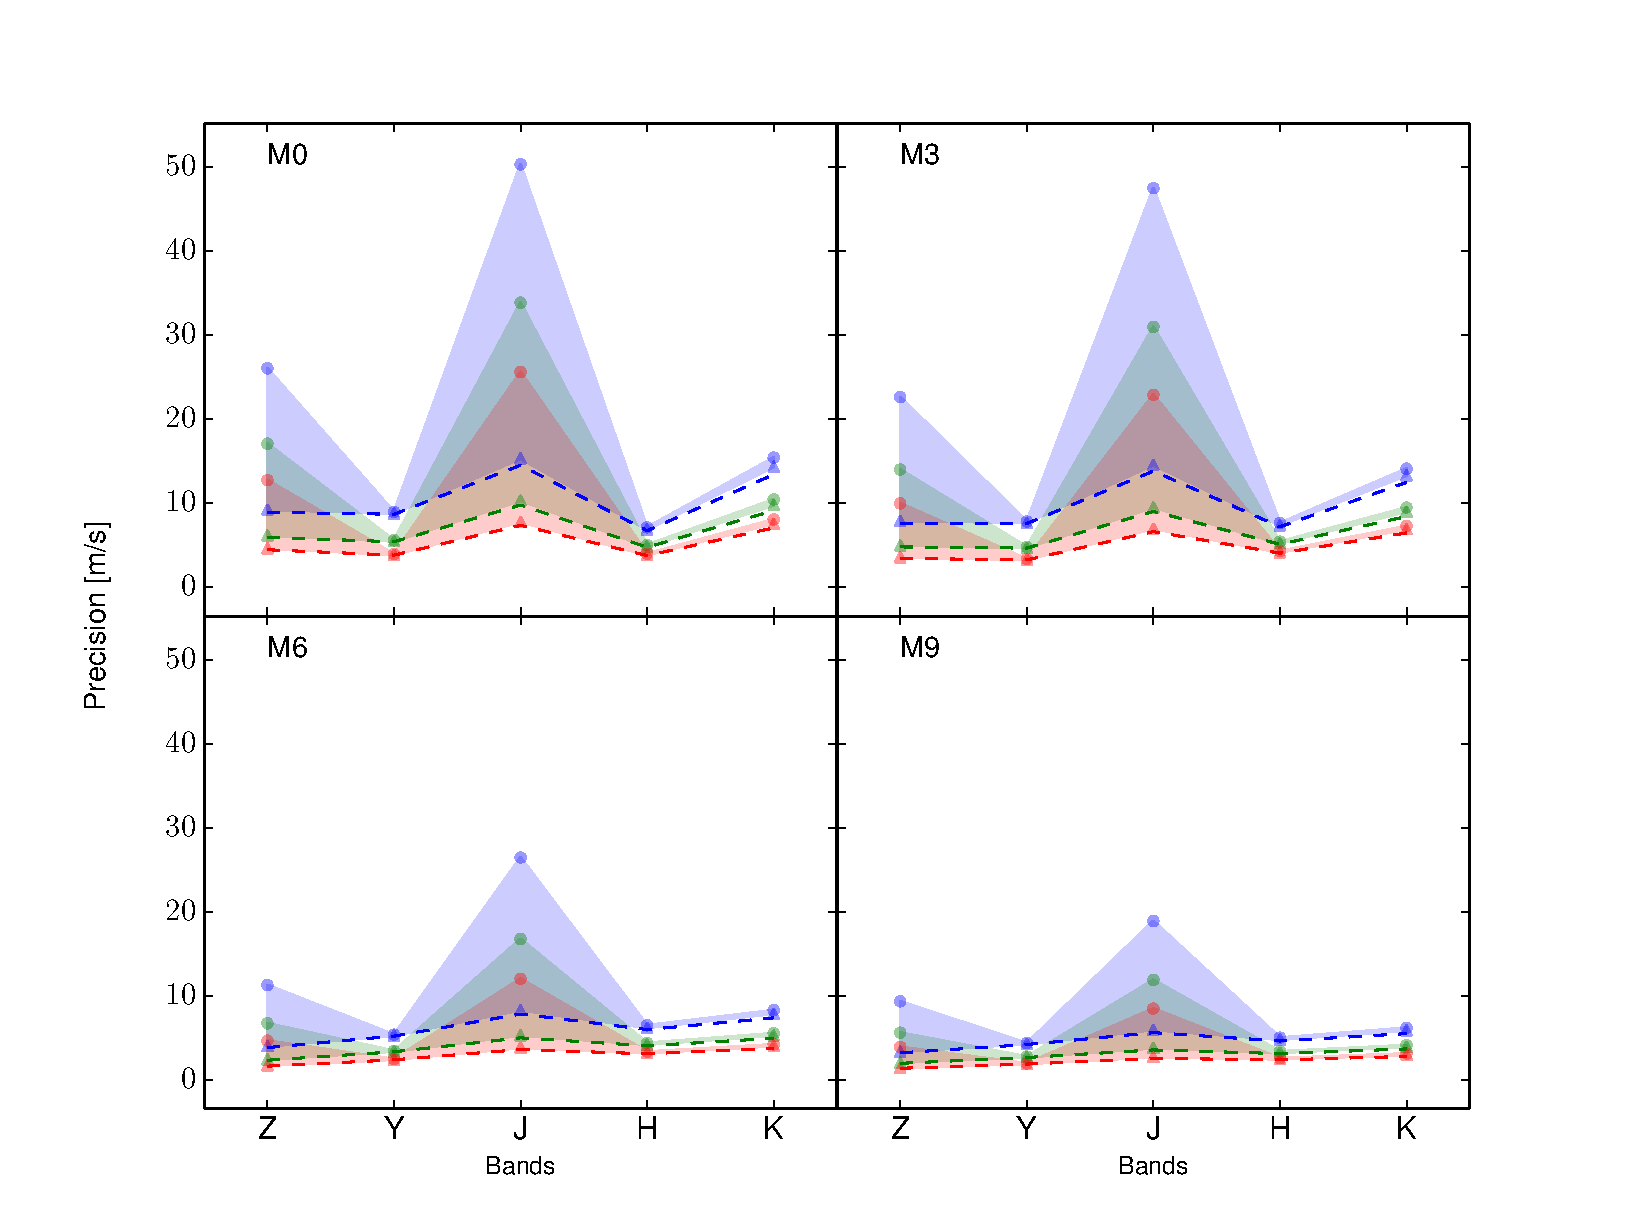
\includegraphics[width=0.48\linewidth]{figures/information-content/Rvprec_vsini1.pdf} &  % Figueria plot
    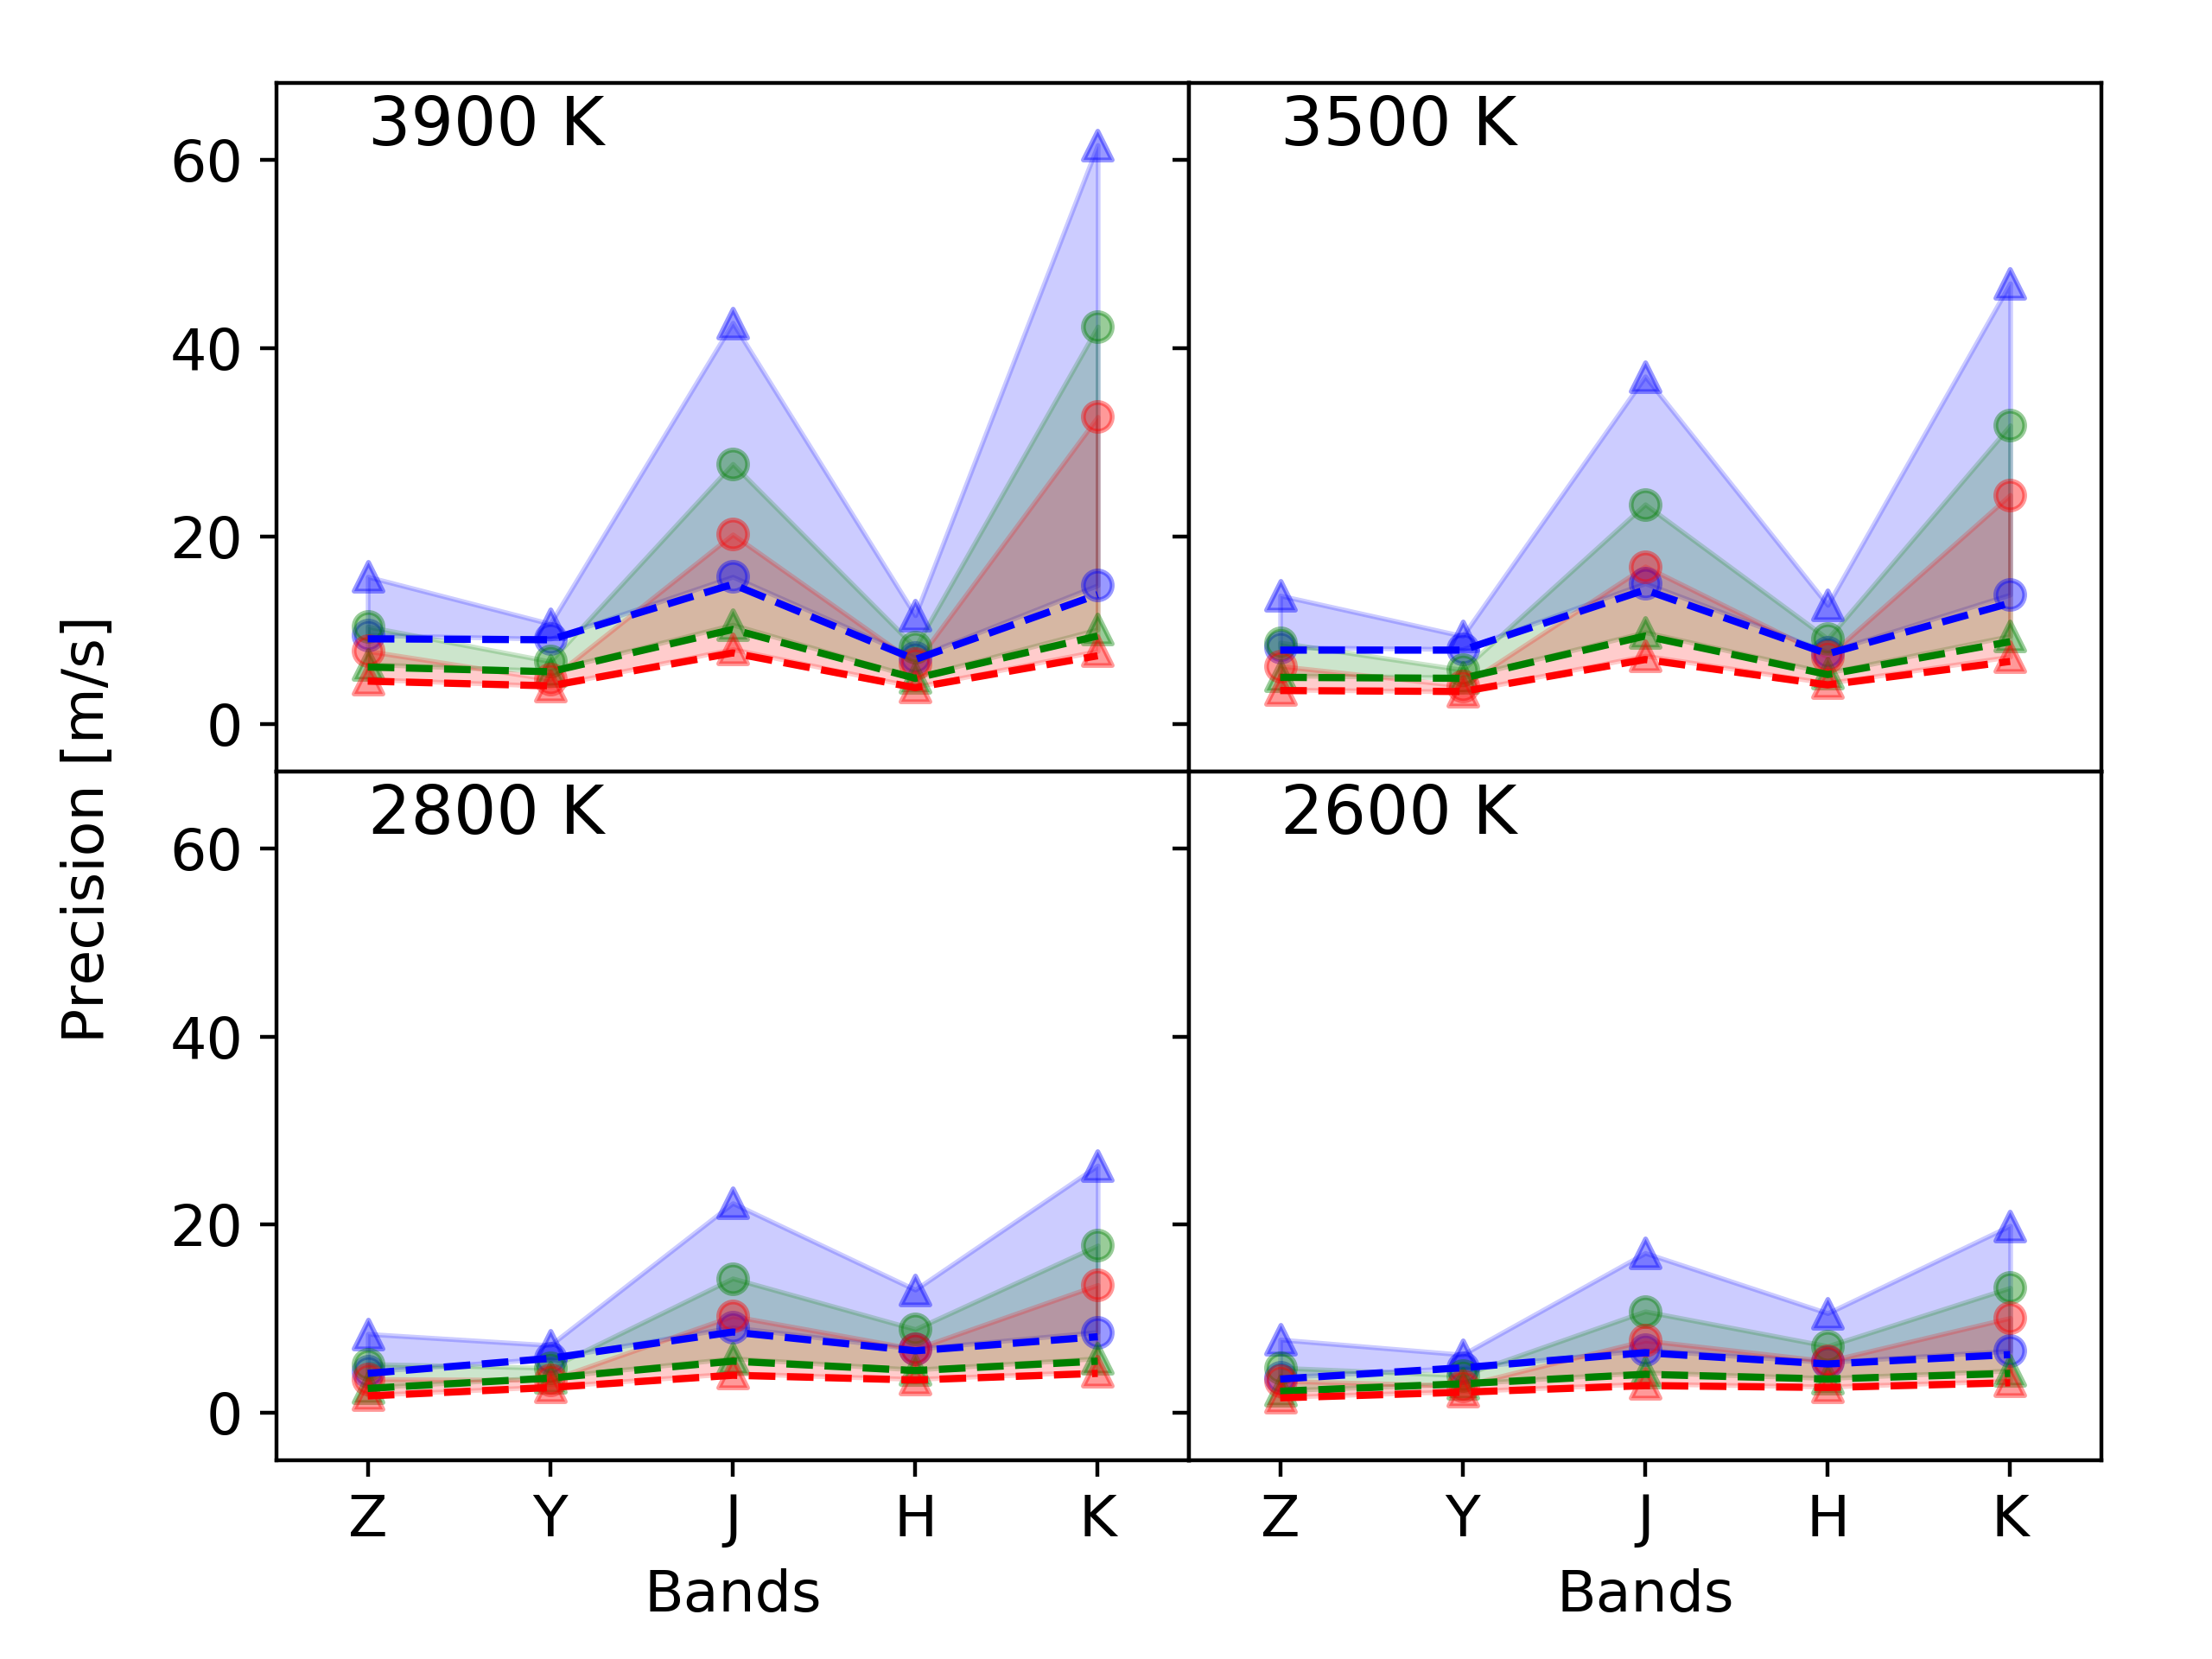
\includegraphics[width=0.47\linewidth]{figures/information-content/precision_fourpanel.png}\\ % eniric plot
    \end{tabular}
    \caption[Comparision of RV precision results to~\citet{figueira_radial_2016}.]{Left: Figure 1 from~\citet{figueira_radial_2016}, Right: The same style figure with values updated from this work, computed with \emph{eniric}.
The main difference is the area of shaded region due to the problem with Condition~\#2 (which is the upper edge).}
    \label{fig:my_label}
\end{figure}
\todo{Change to 55 m/s upper limit?}

\section{ metalicity / \logg{} extension}



\section{Application to {CARMENES} spectra}

- target selection

- preparation of observed spectra

- Banards star (artigau 2018 comparision)


This work is work in progress.
So far only 1 of 8 planned {CARMENES} spectra have been telluric corrected to calculate the RV precision.

{I can calculate the rv precision from models though.}
